\documentclass[12pt,letterpaper,english,bibliography=totocnumbered, abstract=on]{scrartcl}

\usepackage{indentfirst}
\usepackage[titletoc]{appendix}
%\usepackage{fullpage}
%\usepackage{subfiles}
\usepackage[T1]{fontenc}
\usepackage[latin9]{inputenc}
\usepackage{color}
\usepackage{babel}
\usepackage{verbatim}
\usepackage[unicode=true,pdfusetitle,
bookmarks=true,bookmarksnumbered=false,bookmarksopen=false,
breaklinks=true,pdfborder={0 0 0},pdfborderstyle={},backref=false,colorlinks=true]
{hyperref}
\hypersetup{linkcolor=blue,citecolor=blue,urlcolor=blue}

\usepackage{booktabs}
\usepackage{multirow}
\usepackage{adjustbox}
\usepackage{threeparttable}
\usepackage[table]{xcolor}
\usepackage{csquotes}
\usepackage{soul} % for hiliting text: \hl

\usepackage[backend=biber, sorting=none]{biblatex}
%\setlength\bibitemsep{2\itemsep}
%\addbibresource{mylibrary.bib}
\addbibresource{CRB.bib}

\usepackage{pdfpages}
\usepackage{float} % Allows use of H to place floats

\usepackage{pgfgantt}

\usepackage{framed}
\usepackage{todonotes}

% Prevent page breaks within paragraphs
% https://tex.stackexchange.com/questions/21983/how-to-avoid-page-breaks-inside-paragraphs
\widowpenalties 1 10000

\begin{document}

\titlehead{Technical Report}

\title{Using a Cell Phone to as a Datalogger for Handheld Harmonic Radar}

\author{Aubrey Moore PhD\\University of Guam College of Natural and Applied Sciences}

\date{\today}

\maketitle

%\begin{footnotesize}
%	\url{https://xxx}
%\end{footnotesize}

\clearpage

For scientific applications, such as tracking tags attached to insects, it is desirable to log output from the hand-held RECCO harmonic radar device along with timestamp, GPS coordinates, direction of signal, intensity of signal, etc. Here, I report on my attempts use a cell phone as a datalogger.

When the RECCO detects a tag, it alerts the user with an audible beeps. The intensity of these beeps indicates the strength of the returned signal and the direction of the tag is in line with the Yagi antenna.

\section{Materials and Methods}

\subsection{Setting up a Smart Phone}


\subsubsection{Hardware}

I used a Samsung Galaxy 5 smart phone. Beeps were recorded by connecting the phone's audio jack to the headphone plug RECCO. It was necessary to build a simple interface circuit before the phone would record from the audio jack (Fig. \ref{fig:adapter}). This circuit was integrated with a custom made plug for the RECCO headphone jack (Figs. \ref{fig:recco1},\ref{fig:recco2}).

\begin{figure}[p]
	\centering
	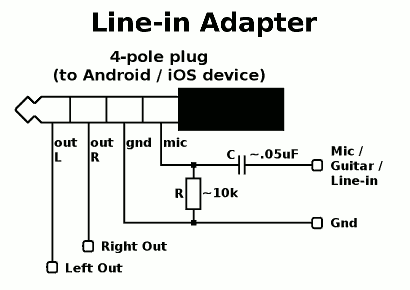
\includegraphics[width=0.7\linewidth]{images/adapter}
	\caption{Line-in adaptor circuit for cell phones. Source: \url{https://warmplace.ru/docs/mobile_audio_input/}}
	\label{fig:adapter}
\end{figure}

\begin{figure}[p]
	\centering
	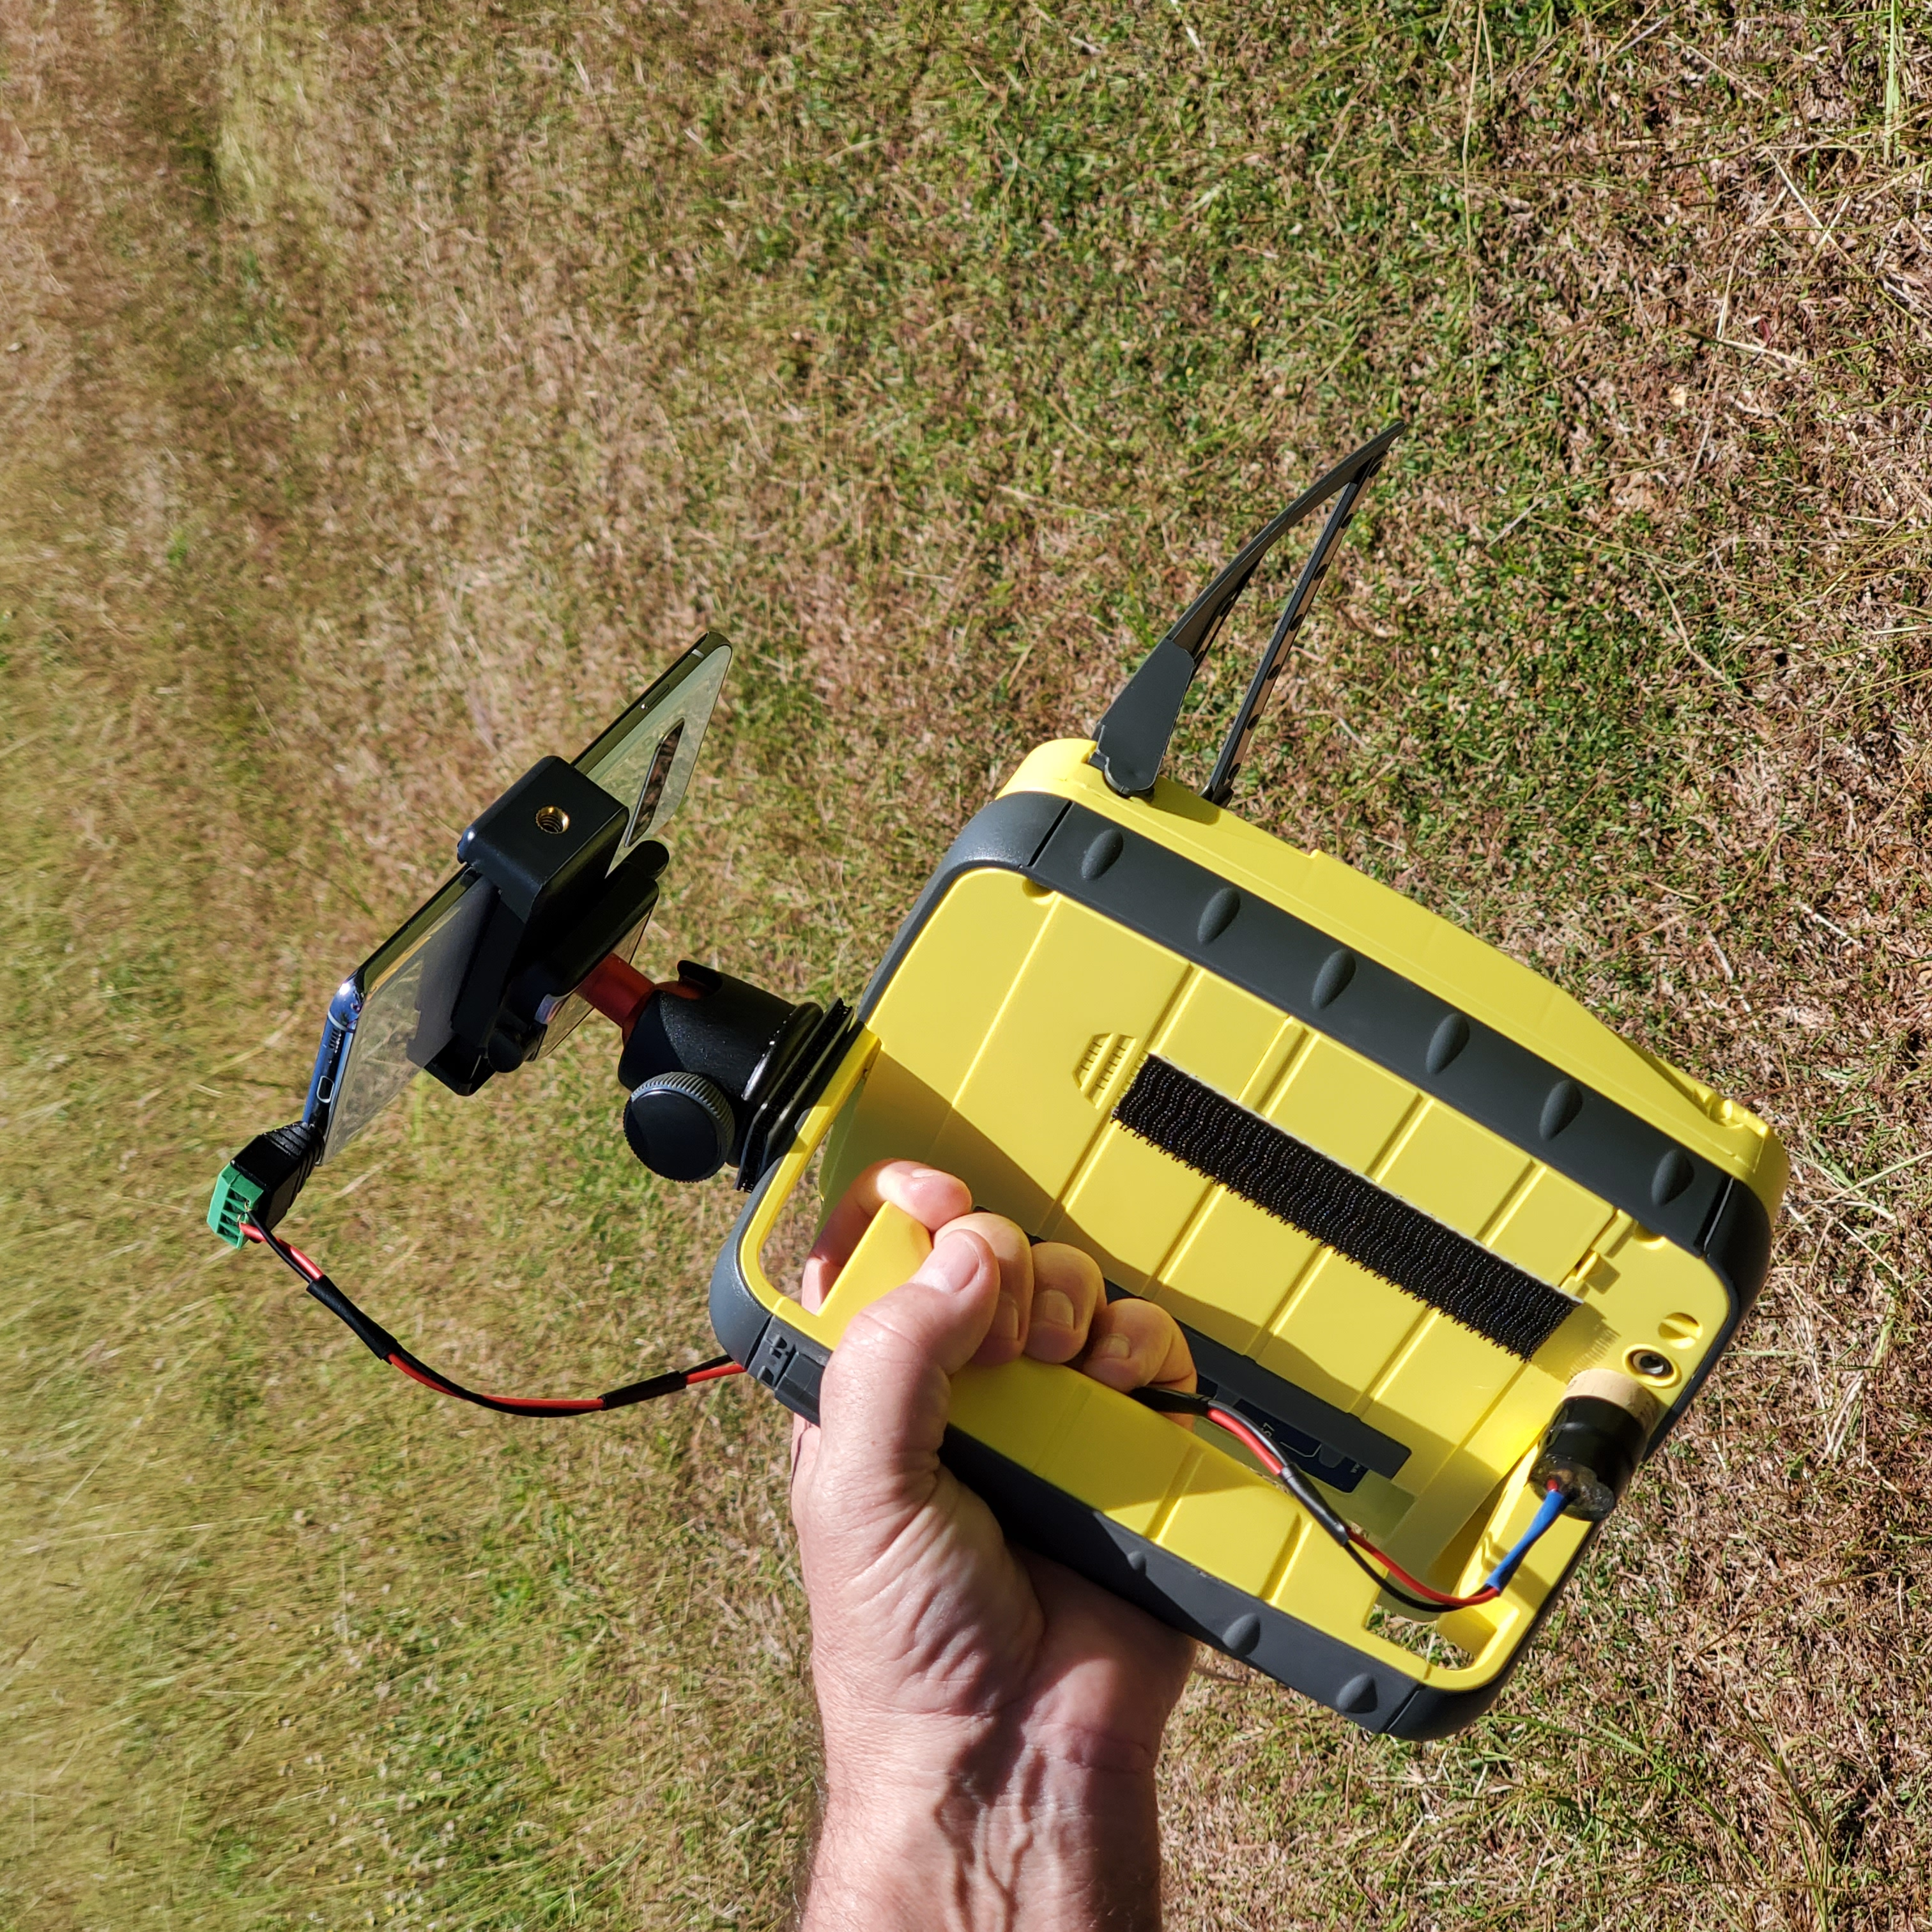
\includegraphics[width=0.7\linewidth,angle=-90]{images/recco1}
	\caption{RECCO hand-held harmonic radar with smart phone attached.}
	\label{fig:recco1}
\end{figure}

\begin{figure}[p]
	\centering
	\includegraphics[width=0.7\linewidth,angle=-90]{images/recco2}
	\caption{RECCO hand-held harmonic radar with smart phone attached.}
	\label{fig:recco2}
\end{figure}


The phone was attached on top of the RECCO's handle using a ball mount and phone holder (Figs. \ref{fig:recco1},\ref{fig:recco2}).

\subsubsection{Software}

I used a free \href{https://www.arduino.cc/education/science-journal}{Arduino Science Journal app}. This app allows selection of various sensors for recording experimental data.  In this case, I used the sound intensity sensor, and the compass direction sensor.

\subsection{Field Test}

Prior to connecting the phone to the REVCCO, I \href{https://www.howtogeek.com/519142/how-to-calibrate-the-compass-on-android-to-improve-device-location-accuracy/}{calibrated the compass sensor}.

A RECCO test tag was clamped to a tripod at about 1.5 m above ground at one end of a small field Fig. (\ref{fig:target}). At the other end of the field, 70 m away (Fig.\ref{fig:screenshot-from-2021-02-22-08-47-24}), I made several counter clockwise rotations while holding the RECCO with smart phone as in Fig. \ref{fig:recco2}.

\begin{figure}[p]
	\centering
	\includegraphics[width=0.4\textwidth, angle=-90]{"images/target"}
	\caption{RICCO test target containing a harmonic radar tag.}
	\label{fig:target}
\end{figure}

\begin{figure}[p]
	\centering
	\includegraphics[width=0.7\linewidth]{"images/Screenshot from 2021-02-22 08-47-24"}
	\caption{Test setup. The line shows the 70m distance between the RECCO harmonic rader device on the left and the test target tag on the right.}
	\label{fig:screenshot-from-2021-02-22-08-47-24}
\end{figure}


\section{Analysis and Results}

The CSV data file recorded by the Arduino Science Journal app was downloaded to my laptop computer and analysed using a Jupyter notebook (see Figs. \ref{fig:compass},\ref{fig:decibels},\ref{fig:polar0},\ref{fig:polar75}).

\begin{figure}[p]
	\centering
	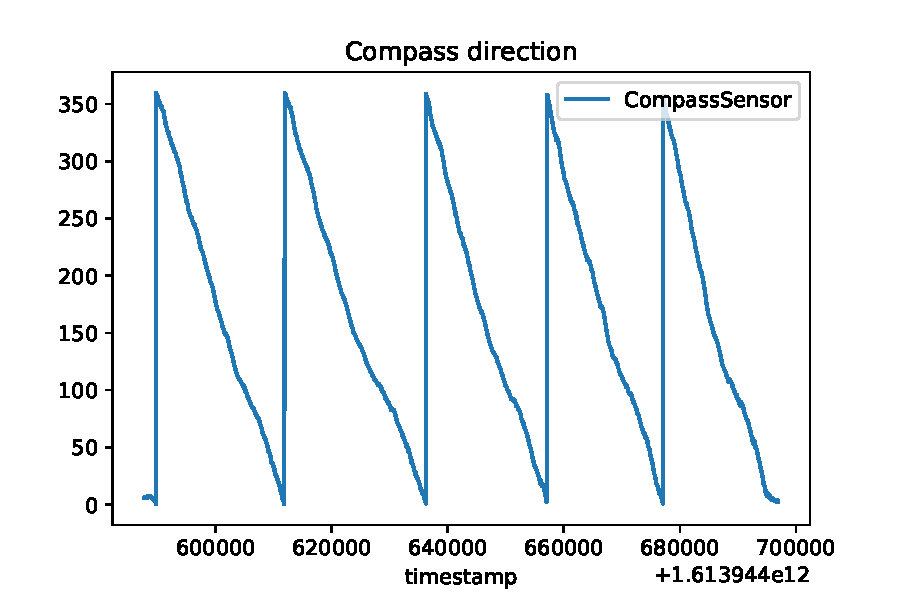
\includegraphics[width=0.7\linewidth]{images/compass}
	\caption{Compass direction.}
	\label{fig:compass}
\end{figure}

\begin{figure}[p]
	\centering
	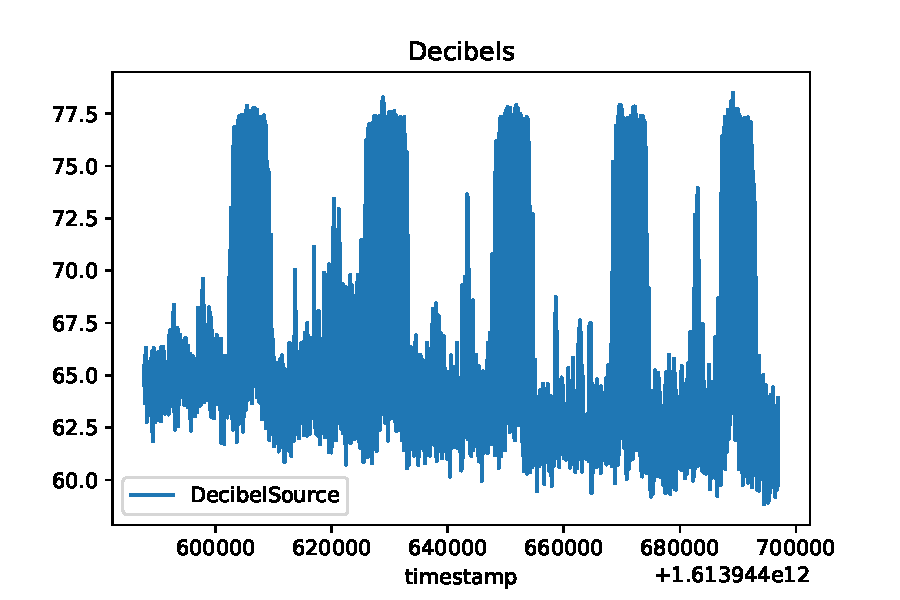
\includegraphics[width=0.7\linewidth]{images/decibels}
	\caption{Sound intensity.}
	\label{fig:decibels}
\end{figure}

\begin{figure}[p]
	\centering
	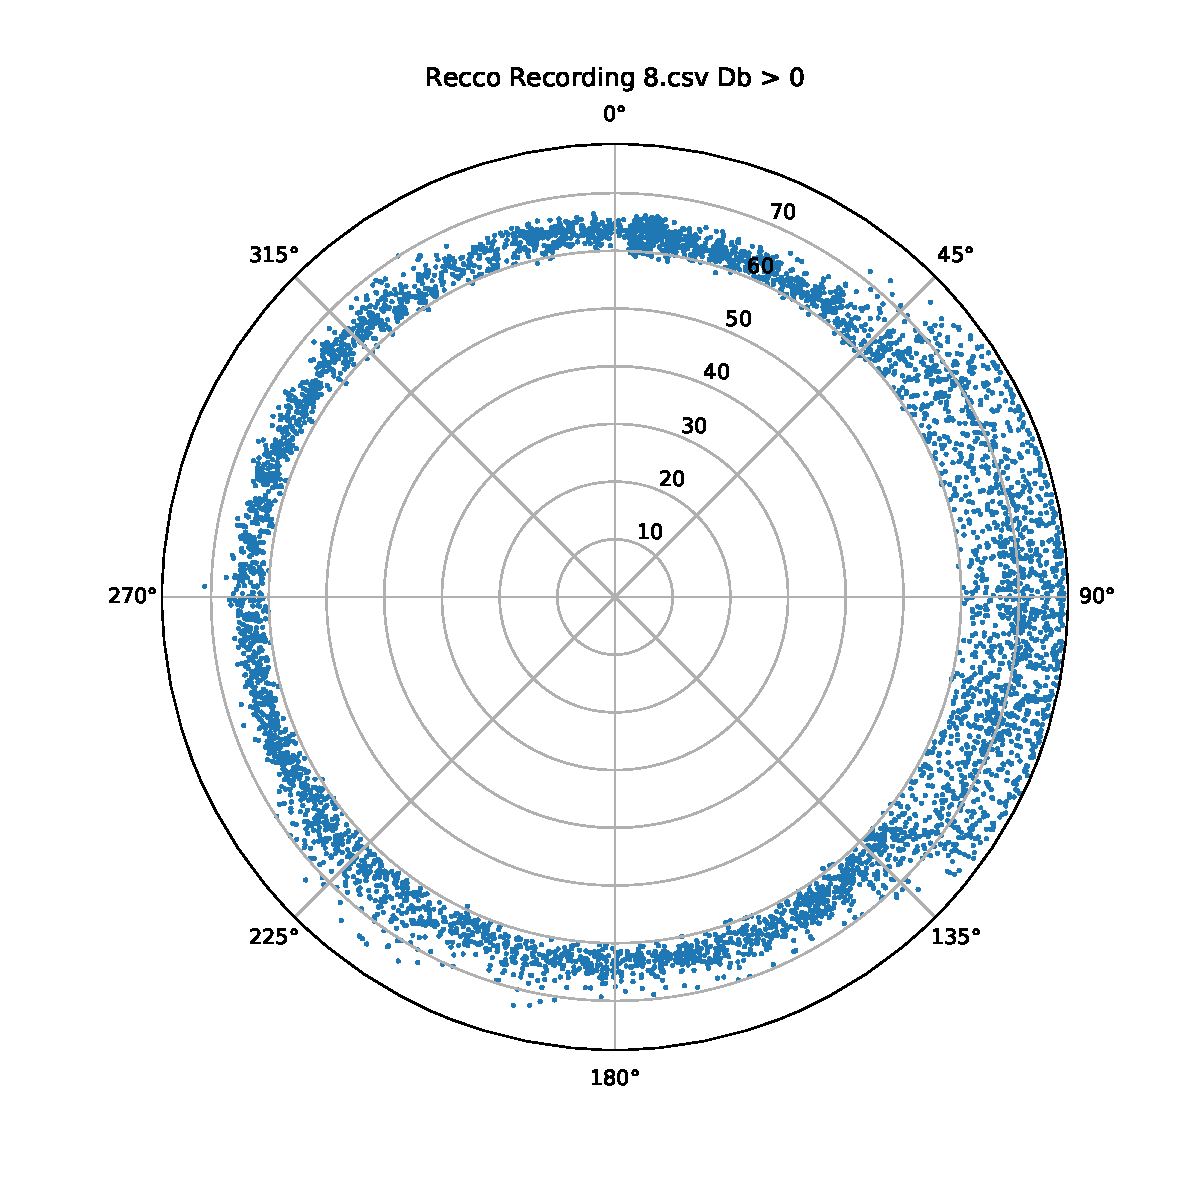
\includegraphics[width=0.7\linewidth]{images/polar0}
	\caption{Polar plot of sound intensity versus compass direction.}
	\label{fig:polar0}
\end{figure}

\begin{figure}[p]
	\centering
	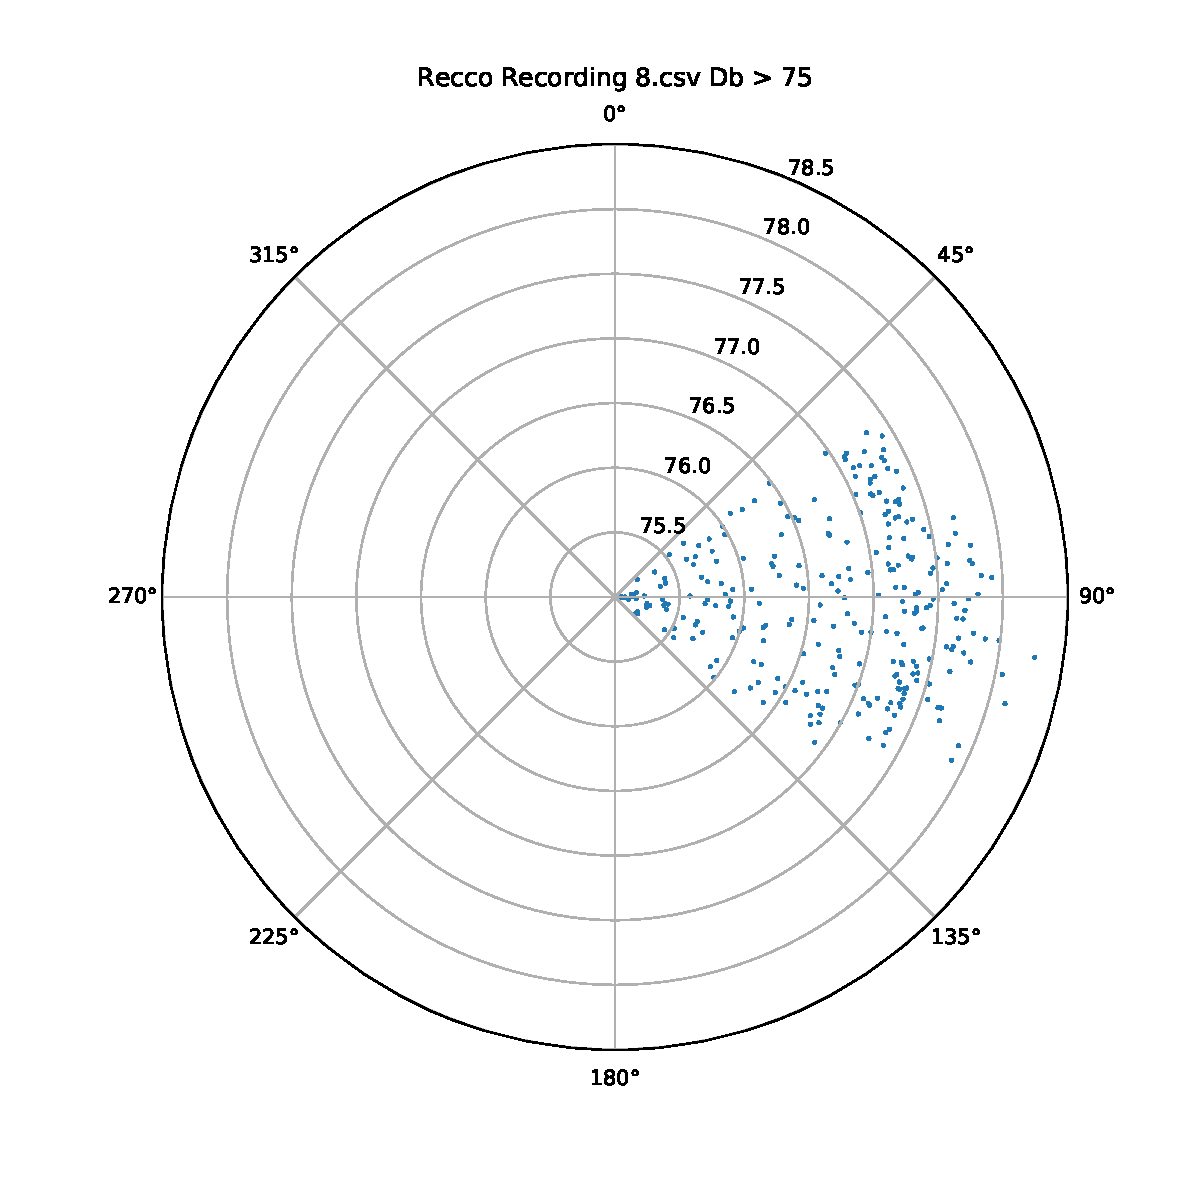
\includegraphics[width=0.7\linewidth]{images/polar75}
	\caption{Polar plot of sound intensity versus compass direction.}
	\label{fig:polar75}
\end{figure}

\section{Discussion}

All of the signals above 75 dB were from the east quadrant, centered on the location of the test tag (Fig. \ref{fig:polar75}).

The beeps are on top of a very loud (60 dB to 70 dB)white noise background. It should be possible to increase the  signal-to-noise ratio significantly by recording the raw waveform (as a WAV file) instead of calculating decibels integrated over all frequencies. A spectral filter could then be used to ignore everything except the beep frequency.

\end{document}
